\chapter{Combining RL and Auto-regression}
\label{chap:RL-Autoregression}

Reinforcement learning is the top-level framework for AGI.  Auto-regressive learning such as for LLMs is the current state-of-the-art technique to produce near-human-level intelligence.  This success is a ``first approximation'' of the success we ultimately want.  How can we combine reinforcement learning with auto-encoders to create true AGI?

The essence of auto-regressive learning or auto-encoder:
\begin{equation}
	\vcenter{\hbox{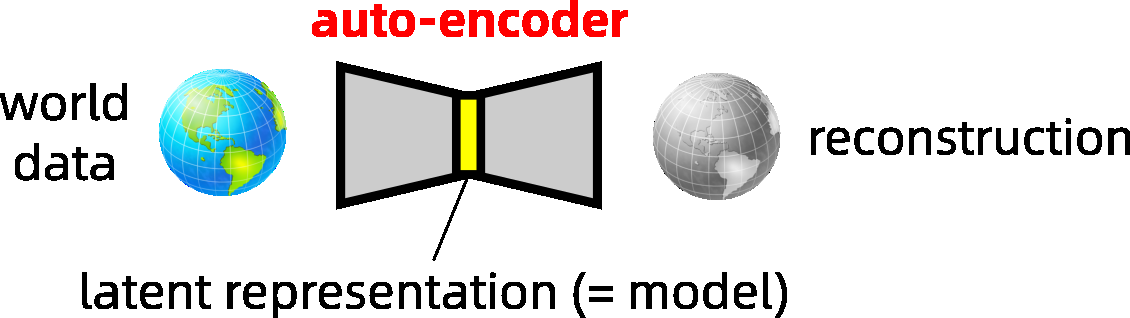
\includegraphics[scale=0.5]{auto-encoder.png}}}
\end{equation}
The corpus data currently in use for training LLMs can be viewed in two ways:
\begin{description}
	\item[\hspace{2em} case (A)] the corpus data represent ``the world'': \\
	world state \autoencoder next state
	\item[\hspace{2em} case (B)] the corpus data represent samples of human thought-processes: \\
	thought \autoencoder next thought
\end{description}
Both views seem to be effective for training AGIs.  In both cases, the corpus being mostly text-based dictates that LLMs model natural language (obviously).  But this is different from the case of RL.

Next we look at the basic architecture of reinforcement learning:
\begin{equation}
% from /2023/RL-with-world-model.svg and generative-models-and-AGI.svg
\vcenter{\hbox{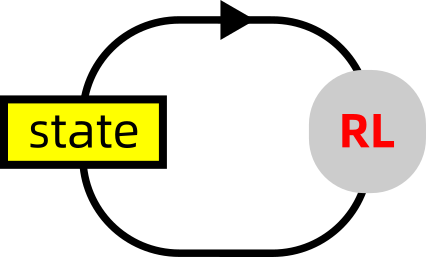
\includegraphics[scale=0.5]{minimal-RL.png}}}
\end{equation}
and see where it ``intersects'' with the auto-encoder.

In case (A), the \textbf{RL state} is a representation of the world, and this representation can increase in accuracy or insights by ``thinking.''  The question is how to reconcile the RL state being in an internal representation form, versus the explicit NL form in an LLM.  

In case (B) the LLM emulates the ``internal'' RL state using explicit NL sentences.

The goal of RL is to maximize the reward:
\begin{equation}
\max_{\pi} \; \underset{\substack{a_t \;\sim\; \pi(\cdot | s_t) \\ s_{t+1} \;\sim\; p(\cdot | s_t, a_t) }} {\mathbb{E}} \left[ \sum_{t} \gamma^t R(s_t, a_t) \right]
\end{equation}

If we use RL to model internal mental states, then each action is an internal next-thought.  In this setting, what does auto-regression, or ``prediction of the next state,'' mean?

\begin{comment}
The following approach may be wrong:
\begin{equation}
% from /2023/RL-with-world-model.svg and generative-models-and-AGI.svg
\vcenter{\hbox{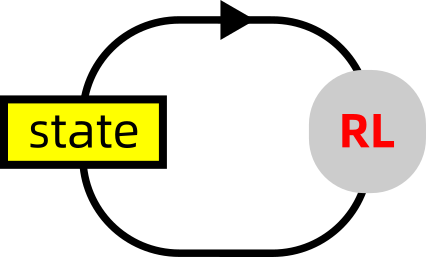
\includegraphics[scale=0.5]{minimal-RL.png}}}
\qquad \qquad
\vcenter{\hbox{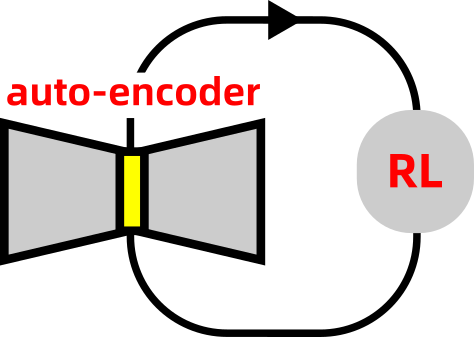
\includegraphics[scale=0.5]{RL-with-autoencoder.png}}}
\end{equation}

The following approach to Tic-Tac-Toe may be wrong:
\begin{equation}
\vcenter{\hbox{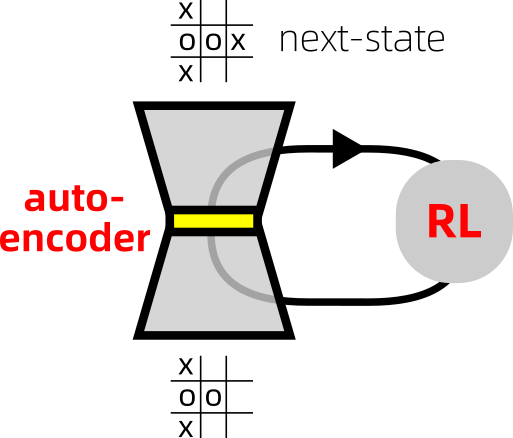
\includegraphics[scale=0.7]{RL-with-autoencoder-TTT.png}}}
\end{equation}
What we call ``prediction'' should be about external world-states.  

\end{comment}

Think about it:  it does not make too much sense for auto-regression to predict the next \textit{internal} thought;  that would be highly redundant.

\begin{equation}
\vcenter{\hbox{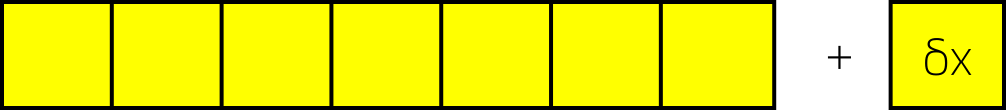
\includegraphics[scale=0.7]{state-with-delta.png}}}
\end{equation}

